\documentclass[12pt]{article}
\usepackage{ctex}
\usepackage{graphicx}
\usepackage{indentfirst}
\usepackage{amsmath}
\usepackage{float}
\usepackage{amssymb}
\usepackage{bm}
\title{第七周作业报告}
\author{佐藤拓未 20300186002}
\date{}


\begin{document}
	
	\maketitle
	
	
	
	
	\begin{center}
		\textbf{第一问}
	\end{center}
	\noindent 证明线性多步方法$u_{n+2}=u_{n+1}+\frac{\Delta{t}}{4}(f_{n+2}+2f_{n+1}+f_n)$是$A_0$-稳定的.\\
	\quad \\
	\noindent \textbf{证明:} 考虑$\rho(\lambda)-z\sigma(\lambda)=0$, 并约去等式两边因子$\lambda^n$, 可知此线性多步方法的绝对稳定区域为$$S=\{z: \lambda^{2}-\lambda-\frac{z}{4}(\lambda^2+2\lambda+1) =0\text{满足根条件} \}$$
	\noindent 进一步整理可得$$S=\{z: (4-z)\lambda^2-2(2+z)\lambda-z=0\text{满足根条件}  \}$$
\noindent 其中$(4-z)\lambda^2-2(2+z)\lambda-z$是关于$\lambda$的二次复系数多项式, 由于考虑线性多步方法是否$A_0$-稳定, 问题转化为: 当$z \in (-\infty,0]$时, 二次多项式的两个根是否满足根条件. \\
经计算可得当$z \in [-\frac{1}{2},0]$时, 二次多项式的根为实数$$\lambda_{1,2}=\frac{2+z \pm 2\sqrt{2z+1} }{4-z}$$
\noindent 考虑$\lambda_1=\frac{2+z+2\sqrt{2z+1}}{4-z}$, 求导并整理可知
\begin{align*}
	\frac{{\rm d}\lambda_1}{{\rm d}z} &= \frac{2z+6\sqrt{2z+1}+10}{(4-z^2)\sqrt{2z+1}} \ge 0, \quad \quad z \in [-\frac{1}{2},0]
\end{align*}
\noindent 从而在区间$[-\frac{1}{2},0]$上, $\lambda_1$在$z=0$取极大, 在$z=-\frac{1}{2}$取极小: $\lambda_1(0)=1,\lambda_1(-\frac{1}{2})=\frac{1}{3}$.\\
当$z\in(-\infty,-\frac{1}{2}]$, $\lambda_1$为虚根, 则经计算可知其模函数为$$\vert \lambda_1(z) \vert=\frac{\sqrt{z^2-4z}}{4-z}$$
\noindent 对其求导有
\begin{align*}
	\frac{{\rm d}\vert \lambda_1\vert}{{\rm d}z} &= \frac{-8+2z}{(4-z^2)\sqrt{z^2-4z}} \le 0,\quad \quad z\in(-\infty,-\frac{1}{2}]
\end{align*}
\noindent 那么可知$\vert  \lambda_1\vert$在区间$(-\infty,-\frac{1}{2}]$上, 在$z\rightarrow -\infty$取极大: $\vert  \lambda_1(-\infty)\vert=1$. \\
再考虑$\lambda_2=\frac{2+z-2\sqrt{2z+1}}{4-z}$, 求导可知
\begin{align*}
	\frac{{\rm d}\lambda_2}{{\rm d}z} &= \frac{-2z+6\sqrt{2z+1}-10}{(4-z^2)\sqrt{2z+1}}\\
	&\le \frac{-4}{(4-z^2)\sqrt{2z+1}}\le0, \quad \quad z \in [-\frac{1}{2},0]
\end{align*}
\noindent 可知在区间$[-\frac{1}{2},0]$上, $\lambda_2(0)=0$取极小, $\lambda_2(-\frac{1}{2})=\frac{1}{3}$取极大. 而当$(-\infty,-\frac{1}{2}]$时, 由于$\vert \lambda_2\vert=\vert \lambda_1\vert$, 故此时在$z=-\infty$取模最大值: $\vert \lambda_2(-\infty)\vert=1$.\\
最后, 发现$\lambda_{1,2}$只在无穷远点$z=-\infty$时的模同时为$1$, 由于两个根的表达式不同, 故二次多项式不会在单位圆盘上取到重根.
综上所述, 当$z\in(-\infty,0]$时, 二次多项式$(4-z)\lambda^2-2(2+z)\lambda-z$满足根条件, 因此负实轴包含在绝对稳定区域$S$当中, 从而线性多步方法是$A_0$-稳定的.
	
	
	
	
\quad	\\
	\begin{center}
		\textbf{第二问}
	\end{center}


\noindent 考虑如下方程:$$\frac{{\rm d}u}{{\rm d }t}=\lambda(-u+\cos (t))$$
取初值为$u(0)=0$或$1$.\\
\quad \\
$(1)$写出精确的$u(t)$表达式:\\
$(2)$对$\lambda=1,10,100,1000$, 分别用显式Euler格式和隐式Euler格式求解:
$(3)$比较用Adams方法和Gear方法计算$\lambda=1000$时的数值行为.\\
\quad\\
\noindent \textbf{解:}\\
(1): 可知$u^{'} + \lambda u=\lambda \cos (t) $, 则$(e^{\lambda t}u(t))^{'}=\lambda e^{\lambda t}\cos (t)$\\
求解可得$$u(t)=Ce^{-\lambda t}+\frac{\lambda}{1+\lambda^2}(\sin (t)+\lambda \cos (t))$$
\noindent 其中$C$为常数. 

若$u(0)=0$:\quad$$u(t)=-\frac{\lambda^2}{1+\lambda^2}e^{-\lambda t}+\frac{\lambda}{1+\lambda^2}(\sin (t)+\lambda \cos (t))$$
\noindent 若$u(0)=1$:\quad$$u(t)=\frac{1}{1+\lambda^2}e^{-\lambda t}+\frac{\lambda}{1+\lambda^2}(\sin (t)+\lambda \cos (t))$$\\
(2): 对于不同的$\lambda$, 想要观察显式Euler与隐式Euler格式的末项收敛阶, 以此观察两格式的收敛性. \\
\underline{当初值$u(0)=0$时}: 令$u(0)=0, t_0=0, T=1, \Delta{t}=2^{-i}, i=2,3,\cdots$, 这样一来, $p$阶方法末项的相对误差对数值与$i$应当是斜率为$-p\ln2$的线性关系.\\
当$\lambda=1$时, 从图1可以看出显式Euler与隐式Euler格式在数值上均为一阶方法. 特别的, 令此时的$\Delta{t}=0.02$, 此时两种Euler格式的精度是相当的, 具体图像见图2.\\
当$\lambda=10$时, 收敛阶与$\lambda_1$的情形类似, 当$i\ge3$时, 两种Euler格式的末项收敛阶均为一阶的. 特别的, 令此时的$\Delta{t}=0.02$, 此时两种Euler格式的精度也是相当的, 具体图像见图4.\\
当$\lambda=100$时, 隐式Euler格式的末项相对误差仍保持着1阶收敛, 但显式Euler格式的收敛情形较差: 此时需要步长$\Delta{t}\le2^{-6}$才能使得末项相对误差一阶收敛, 见图5. 图6展示了当$\Delta{t}=0.02, \lambda=100$的情形: 显式Euler格式的近似解一直在震荡, 这是因为$\lambda=100$时, 显式Euler格式为$u_{n+1}-u_n=2(-u_n+\cos(t_n))$, 进一步整理为$u_{n+1}=-u_n+2\cos(t_n)$,这样的递推式容易引起震荡. 从这例子也可以看出, 由于显式Euler格式是完全取决于上一步的值, 从而当$f$中具有负号、周期函数等时, 迭代格式容易出现较大的误差.\\
当$\lambda=1000$时, 隐式Euler格式仍具有一阶收敛性, 但显式Euler在步长$\Delta{t}=2^{-2}$就已经产生了数值解上的爆破, 具体见图7.
\begin{figure}[H]
	\centering
	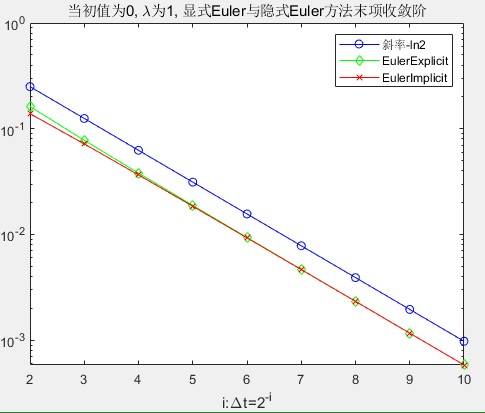
\includegraphics[width=0.75\textwidth]{1}
	\caption{$u(0)=0, \lambda=1$时, 显式Euler与隐式Euler格式的收敛阶}
\end{figure}
\begin{figure}[H]
	\centering
	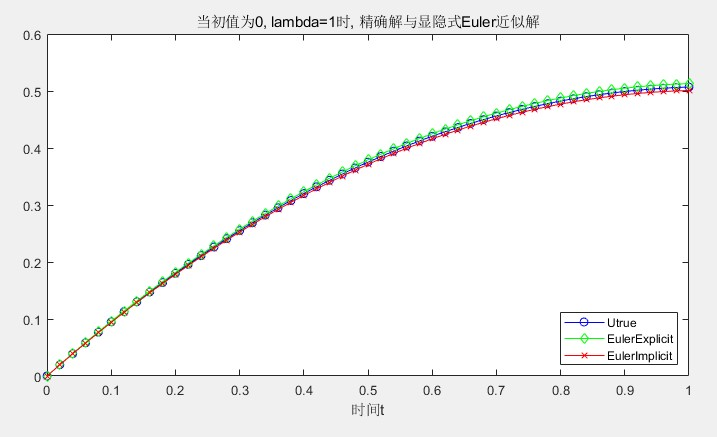
\includegraphics[width=0.75\textwidth]{2}
	\caption{$u(0)=0, \lambda=1,\Delta{t}=0.02$时, 精确解以及显隐式Euler的离散图像}
\end{figure}
\begin{figure}[H]
	\centering
	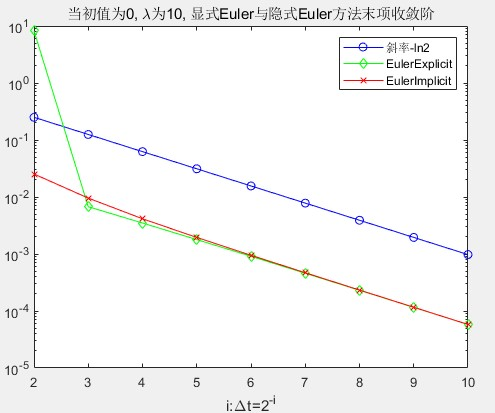
\includegraphics[width=0.75\textwidth]{3}
	\caption{$u(0)=0, \lambda=10$时, 显式Euler与隐式Euler格式的收敛阶}
\end{figure}
\begin{figure}[H]
	\centering
	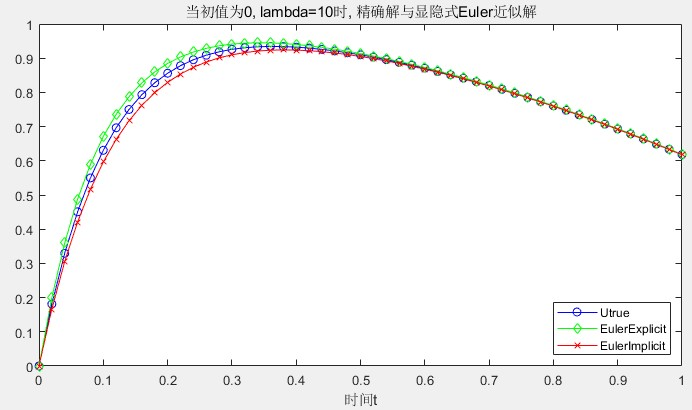
\includegraphics[width=0.75\textwidth]{4}
	\caption{$u(0)=0, \lambda=10,\Delta{t}=0.02$时, 精确解以及显隐式Euler的离散图像}
\end{figure}
\begin{figure}[H]
	\centering
	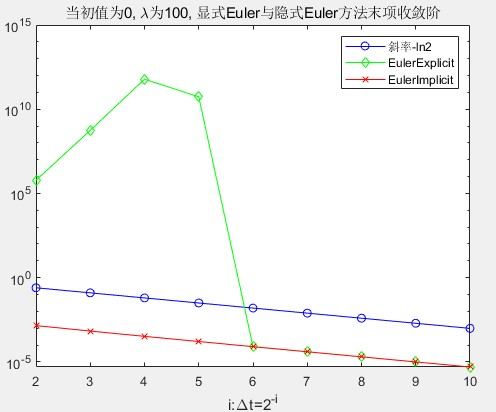
\includegraphics[width=0.75\textwidth]{5}
	\caption{$u(0)=0, \lambda=100$时, 显式Euler与隐式Euler格式的收敛阶}
\end{figure}
\begin{figure}[H]
	\centering
	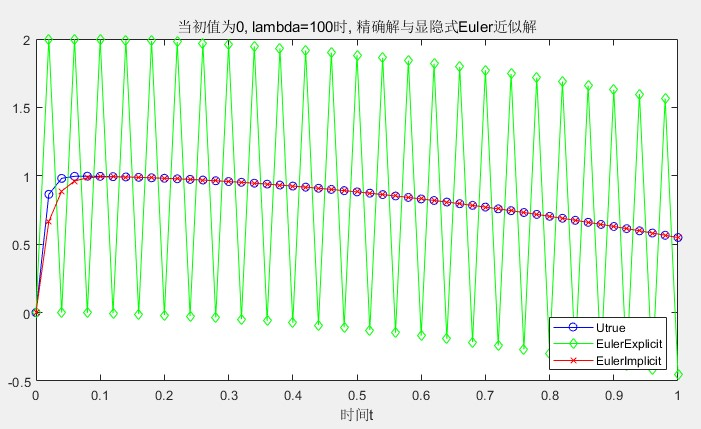
\includegraphics[width=0.75\textwidth]{6}
	\caption{$u(0)=0, \lambda=100,\Delta{t}=0.02$时, 精确解以及显隐式Euler的离散图像}
\end{figure}
\begin{figure}[H]
	\centering
	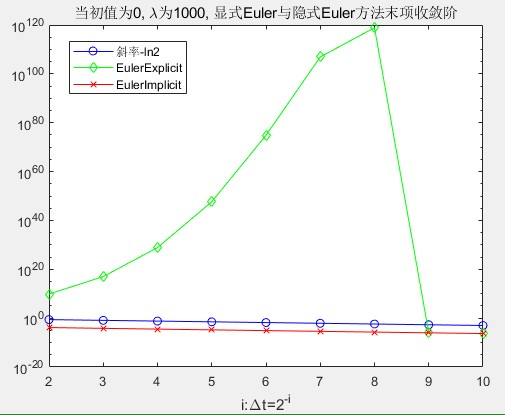
\includegraphics[width=0.75\textwidth]{7}
	\caption{$u(0)=0, \lambda=1000$时, 显式Euler与隐式Euler格式的收敛阶}
\end{figure}

\quad\\

\noindent \underline{当初值$u(0)=1$时}: 仍设$\Delta{t}=2^{-i}$, 并考虑末项相对误差与$i$的关系.\\
当$\lambda=1,10$时, 两种Euler格式的末项相对误差均为一阶收敛的, 具体见图8与图9.\\
当$\lambda=100$时, 隐式Euler仍具有良好的收敛性, 但显式Euler的末项相对误差即便在步长$\Delta{t} \le2^{-6}$后具有一阶收敛性, 但在$\Delta{t}$较大时(例如$2^{-5}$), 通过显式Euler格式求解, 数值解将会爆破.\\
当$\lambda=1000$时, 隐式Euler格式具有良好的一阶收敛性, 但显格式与$\lambda=100$时的情形一致: $\Delta{t}$足够小时具有收敛性, 但当$\Delta{t}$稍大时将会产生数值上爆破, 具体见图12. 特别地, 令$\Delta{t}=0.02$, 会发现显格式在$t_n\ge0.8$时的绝对误差逐渐被放大.
\begin{figure}[H]
	\centering
	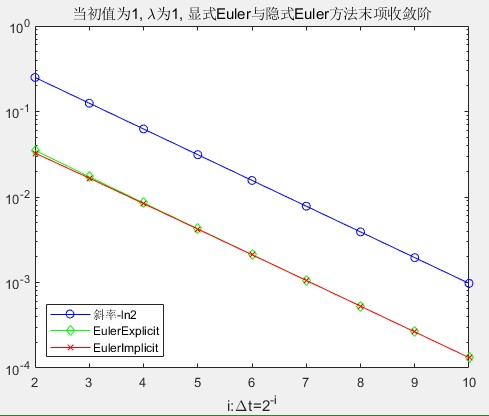
\includegraphics[width=0.75\textwidth]{8}
	\caption{$u(0)=1, \lambda=1$时, 显式Euler与隐式Euler格式的收敛阶}
\end{figure}
\begin{figure}[H]
	\centering
	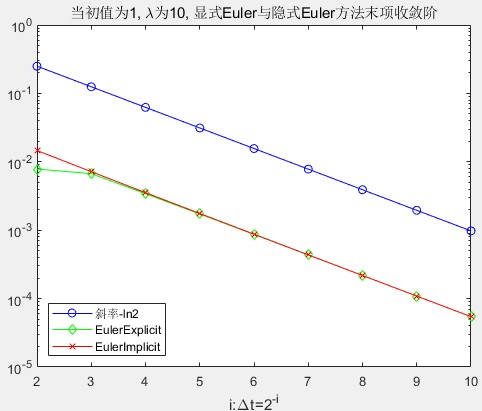
\includegraphics[width=0.75\textwidth]{9}
	\caption{$u(0)=1, \lambda=10$时, 显式Euler与隐式Euler格式的收敛阶}
\end{figure}
\begin{figure}[H]
	\centering
	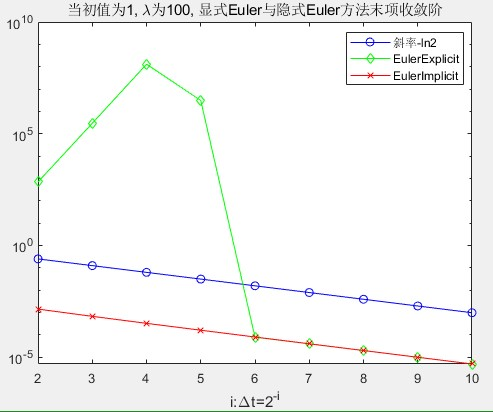
\includegraphics[width=0.75\textwidth]{10}
	\caption{$u(0)=1, \lambda=100$时, 显式Euler与隐式Euler格式的收敛阶}
\end{figure}
\begin{figure}[H]
	\centering
	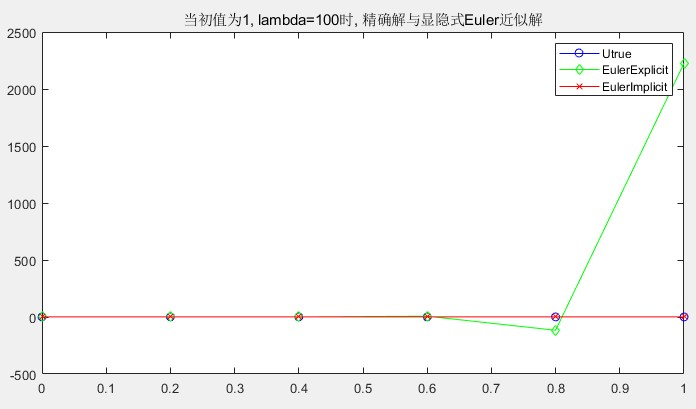
\includegraphics[width=0.75\textwidth]{11}
	\caption{$u(0)=1, \lambda=100,\Delta{t}=0.02$时, 精确解及显隐式Euler的离散图像}
\end{figure}
\begin{figure}[H]
	\centering
	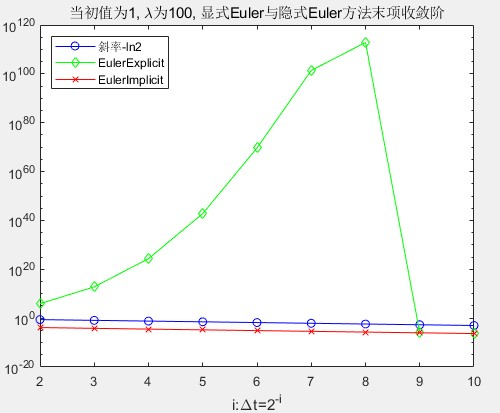
\includegraphics[width=0.75\textwidth]{12}
	\caption{$u(0)=1, \lambda=1000$时, 显式Euler与隐式Euler格式的收敛阶}
\end{figure}
\begin{figure}[H]
	\centering
	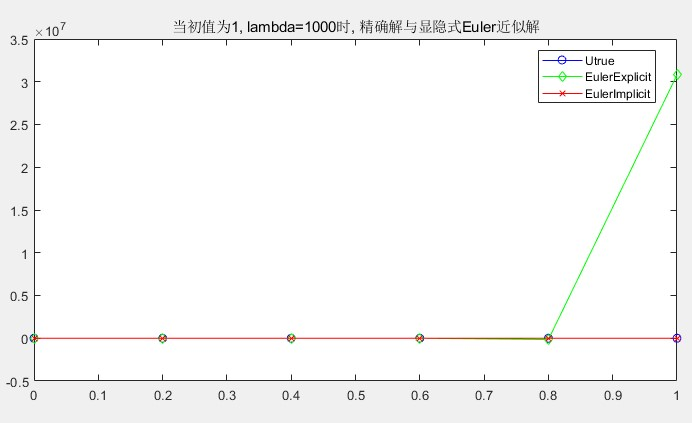
\includegraphics[width=0.75\textwidth]{13}
	\caption{$u(0)=1, \lambda=1000,\Delta{t}=0.02$时, 精确解及显隐式Euler的离散图像}
\end{figure}
\quad \\
\quad \\




\noindent (3): 先考虑四阶方法\\
\underline{当初值$u(0)=0$时}: 此时$\lambda=1000$, 令$\Delta{t}=2^{-i}$, 以此考虑不同格式的收敛阶.\\
此时, Gear4在数值上具有收敛性, 但不具有固定的四阶收敛性, 见图14. 特别地, 令$\Delta{t}=2^{-6}$时, 精确解与Gear四阶格式的离散近似解图像见图15.\\
然而, 如果格式为A-B或A-M四阶格式时, 从它们的收敛阶可以发现它们的末项相对误差在此时具有非常大的误差, 见图16. 造成这样的原因是Adams格式需要取决于前面几步的近似值$f_n$, 由于通过格式计算出来的$u_n$本就与精确值有一定的误差, 又由于$f$的表达式中含有乘积$\lambda$, 故当步长$\Delta{t}$稍大时: $\lambda\Delta{t}\ge1$, 误差会被放大.
\begin{figure}[H]
	\centering
	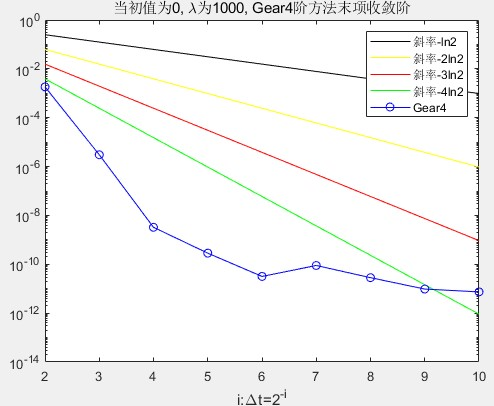
\includegraphics[width=0.75\textwidth]{14}
	\caption{$u(0)=0, \lambda=1000$时, Gear四阶格式的收敛阶}
\end{figure}
\begin{figure}[H]
	\centering
	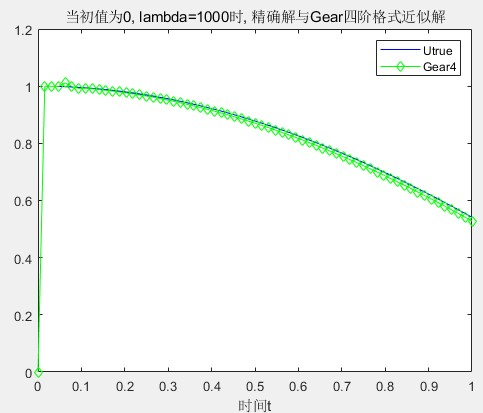
\includegraphics[width=0.7\textwidth]{15}
	\caption{$u(0)=0, \lambda=1000,\Delta{t}=2^{-6}$时, 精确解及Gear4的离散图像}
\end{figure}
\begin{figure}[H]
	\centering
	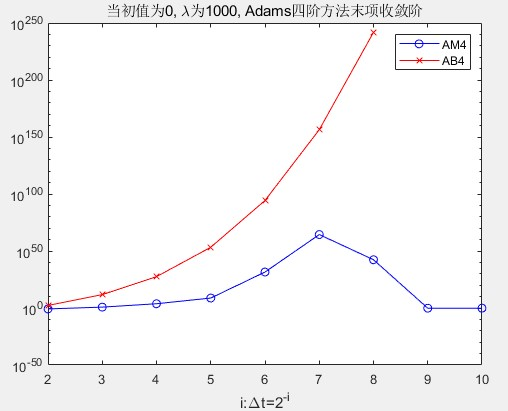
\includegraphics[width=0.7\textwidth]{16}
	\caption{$u(0)=0, \lambda=1000$时, Adams四阶格式的收敛阶}
\end{figure}

\noindent \underline{当初值$u(0)=1$时}: 与$u(0)=0$的情形类似, Gear四阶格式具有收敛性, 但是不是固定四阶收敛性, 见图17. \\
若格式为A-B或A-M四阶格式时, 它们在数值上是不收敛的, 情况与$u(0)=0$的情形非常相似, 见图18.
\begin{figure}[H]
	\centering
	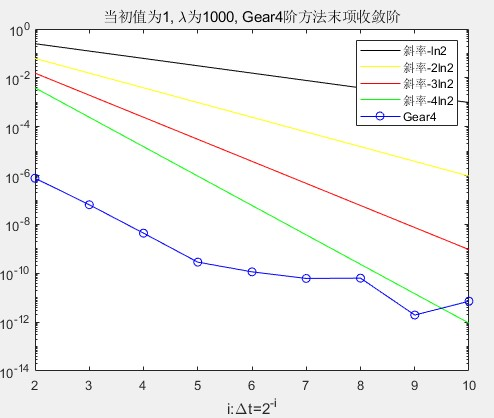
\includegraphics[width=0.75\textwidth]{17}
	\caption{$u(0)=1, \lambda=1000$时, Gear四阶格式的收敛阶}
\end{figure}
\begin{figure}[H]
	\centering
	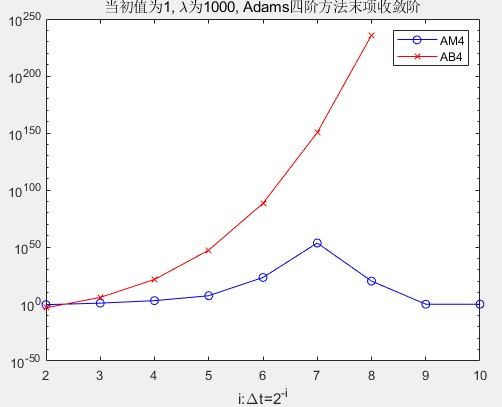
\includegraphics[width=0.75\textwidth]{18}
	\caption{$u(0)=1, \lambda=1000$时, Adams四阶格式的收敛阶}
\end{figure}
\noindent 为了考虑不同阶的A-M与A-B格式是否会对收敛精度产生影响, 考虑对它们降阶.\\
$(3)^{'}:$ 图19中分别展示了当初值$u(0)=0$时的三阶A-M与A-B方法.\\
可以发现A-B与A-M三阶格式均在数值产生了爆破. 然而Gear三阶格式具有固定的三阶收敛性, 其精度要远优于A-B与A-M三阶方法, 具体见图21.\\
\quad \\
我们希望进一步考虑更低一阶的三种格式是否具有稳定性.\\
$(3)^{''}:$ 图22展示了Gear二阶方法的收敛阶, 可以发现Gear二阶格式保持着二阶收敛性; A-M二阶方法退化为改进Euler格式, 此时不在数值上爆破, 其相对误差最终控制在$0.9$以内, 从而并不具有太好的收敛性, 见图23; A-B二阶方法仍然在数值上爆破. 
\begin{figure}[H]
	\centering
	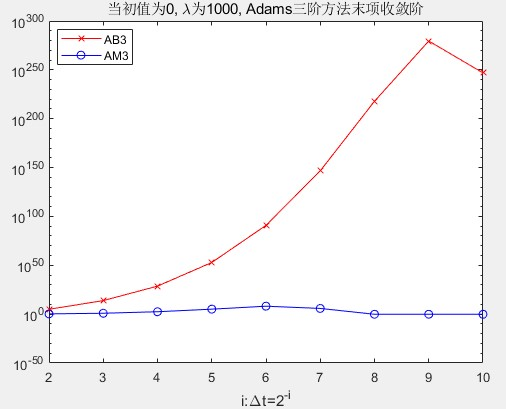
\includegraphics[width=0.72\textwidth]{19}
	\caption{$u(0)=0, \lambda=1000$时, Adams三阶格式的收敛阶}
\end{figure}
\begin{figure}[H]
	\centering
	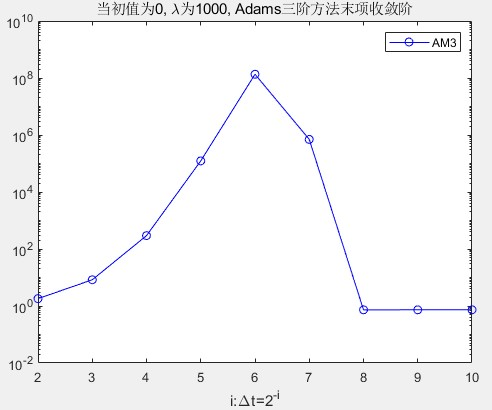
\includegraphics[width=0.72\textwidth]{20}
	\caption{$u(0)=0, \lambda=1000$时, A-M三阶格式的收敛阶}
\end{figure}
\begin{figure}[H]
	\centering
	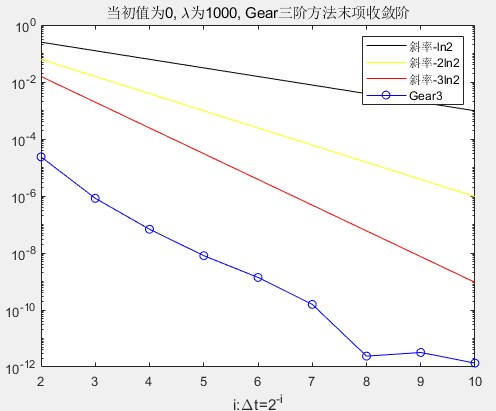
\includegraphics[width=0.72\textwidth]{21}
	\caption{$u(0)=0, \lambda=1000$时, Gear三阶格式的收敛阶}
\end{figure}
\begin{figure}[H]
	\centering
	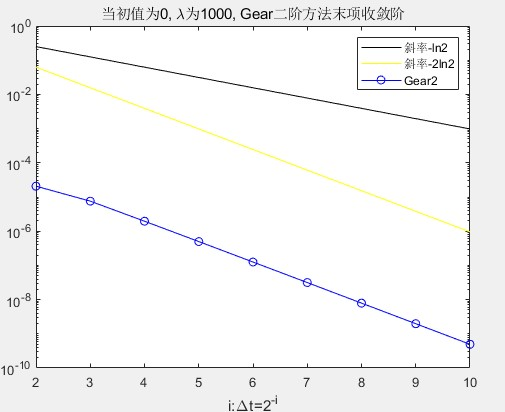
\includegraphics[width=0.72\textwidth]{22}
	\caption{$u(0)=0, \lambda=1000$时, Gear二阶格式的收敛阶}
\end{figure}
\begin{figure}[H]
	\centering
	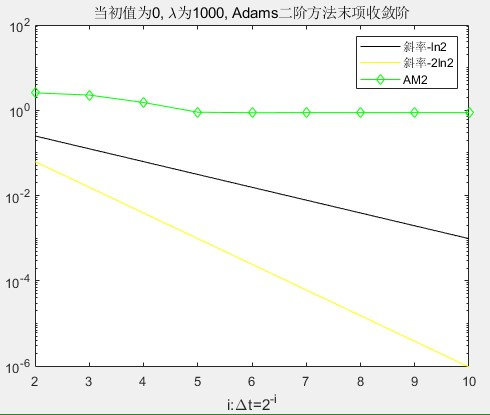
\includegraphics[width=0.72\textwidth]{23}
	\caption{$u(0)=0, \lambda=1000$时, A-M二阶格式的收敛阶}
\end{figure}
\begin{figure}[H]
	\centering
	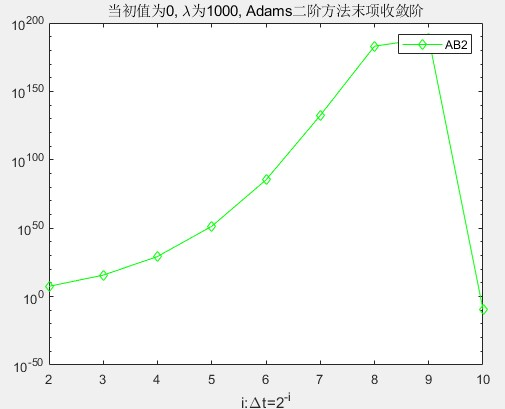
\includegraphics[width=0.71\textwidth]{24}
	\caption{$u(0)=0, \lambda=1000$时, A-B二阶格式的收敛阶}
\end{figure}

\noindent 综合上面的讨论, 可以知道Gear二至三阶格式具有相对应的收敛阶, 而Gear四阶格式虽然不具有固定的四阶收敛阶, 但其仍然具有收敛性, 即Gear格式二至四阶格式在处理此问题具有较优越的收敛性; 对于A-B与A-M二至四显格式而言, 它们的收敛性相较于Gear格式都非常差.\\
A-M与A-B格式在解决此类题目并不具有较好的收敛性是因为: 1) 它们的绝对稳定区域随着方法阶数升高而减少; 2) 无论是A-M格式还是A-B格式, 它们的格式中包含了若干$f_n$项, 而由于$\lambda$的值较大, 从而这些格式的误差会被进一步方法.\\
Gear格式具有较好的收敛性是因为: 1) 它的绝对稳定区域随着阶数增高而增加; 2) Gear格式中只有一项$f_{n+1}$, 且由于Gear格式要求解一次非线性方程, 从而在一定程度上保证了其收敛性.
\end{document}